\section{Gestione dell'I/O}
I computer moderni, secondo il modello di Von Neumann, hanno la CPU e i controller hardware connessi direttamente alla memoria principale del sistema.

Per ogni dispositivo hardware esiste un \textbf{controller}. Il sistema operativo ha poi un \textbf{driver} per ogni controller in grado di leggere i dati dal dispositivo e riportarlo in un formato standard.
\begin{figure}[H]
    \centering
    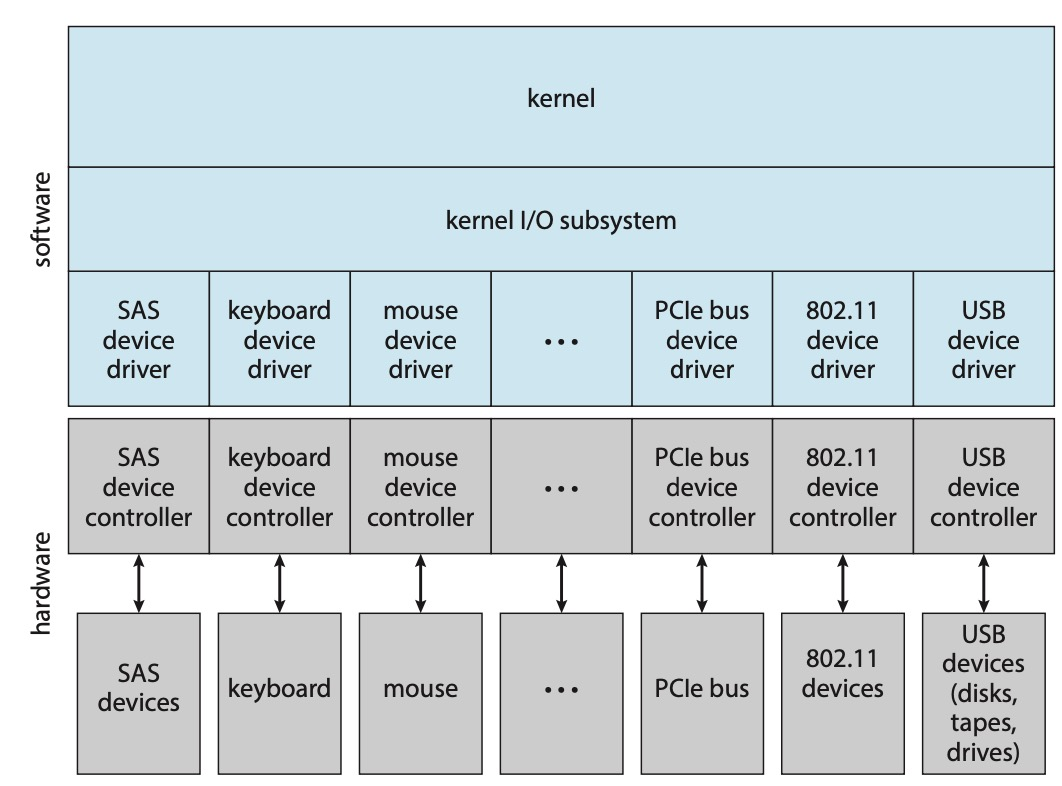
\includegraphics[width=0.45\linewidth]{assets/controller-driver.jpg}
\end{figure}

\begin{note}
    Una cospicua percentuale del codice di un sistema operativo è dedicato alla gestione di I/O, questo per la grande importanza di questi dispositivi rispetto alle prestazioni e l'affidabilità del sistema, inoltre c'è una grande variabilità tra i  vari dispositivi.
\end{note}

\subsection{Interfaccia Comune}
Uno dei compiti del sistema operativo consiste nel nascondere all'utente le caratteristiche dei dispositivi di I/O

Questo viene fatto grazie ad una serie di strategie:
\begin{sitemize}
    \item Il \textbf{Buffering}, ovvero l'uso di un'area di memoria temporanea per immaganizzare dei dati.

    Per esempio la CPU può inserire dei dati in un buffer in attesa che vengano scritti sul disco.
    \item Il \textbf{Caching} consiste nel conservare temporaneamente delle copie dei dati frequentemente utilizzati, anche questa tecnologia viene ampiamente utilizzata nei dispositivi di archiviazione.
    \item Lo \textbf{Spooling} è una tecnica che consiste nell'inserire le richieste di I/O in una coda che viene poi gestita in modo sequenziale.

    Questo consente di gestire più attività contemporaneamente, permette inoltre di continuare l'esecuzione dei programmi del sistema operativo.

    \item Un'\textbf{Interfaccia} generale per i dispositivi.
\end{sitemize}

\subsection{Interrupt}
Un interrupt è il metodo che un dispositivo hardware ha per comunicare con il suo driver.

\spacer
Quando un interrupt si verifica il sistema cerca nel vettore degli interrupt l'indirizzo della subroutine che ha il compito di gestirlo.
Successivamente salva lo stato dell'istruzione interrotta e trasferisce il controllo alla subroutine.

\spacer
Durante la gestione di un interrupt, altri eventuali interrupt giunti al sistema sono momentaneamente “disabilitati”.

\spacer
Gli interrupt sono spesso utilizzati nella gestione dei dispositivi I/O per la loro semplicità, tuttavia quando un dispositivo ha necessità di trasferire grandi quantità di dati l'utilizzo di interrupt può rallentare in modo significativo il sistema.

\begin{figure}[H]
    \centering
    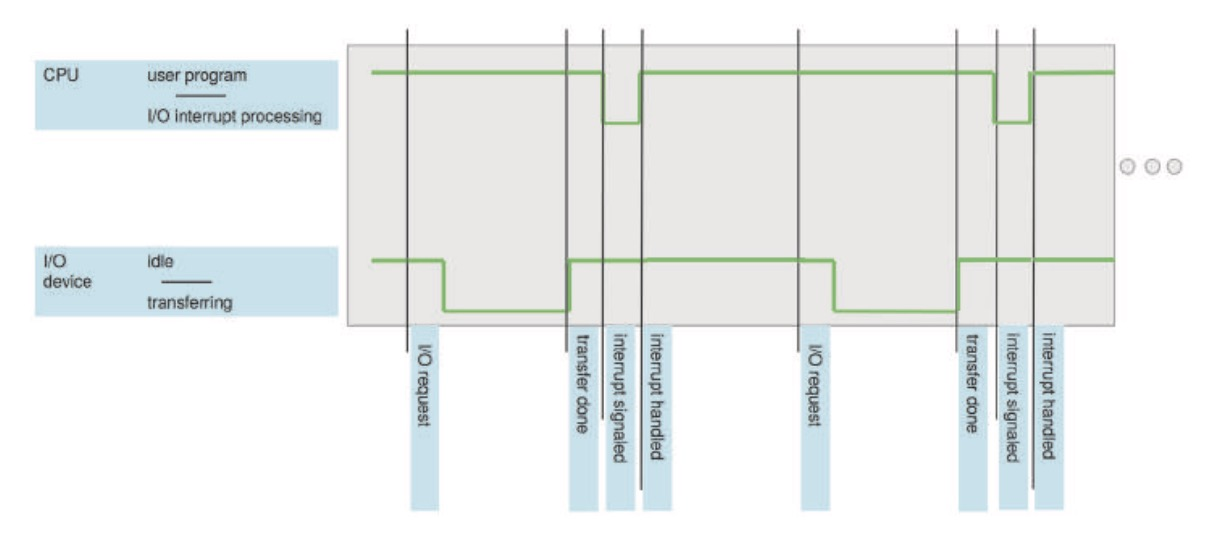
\includegraphics[width=0.65\linewidth]{assets/interrupt-timeline}
    \caption{Timeline per un interrupt}
\end{figure}

\subsubsection{Interrupt sincrono}
È l'implementazione più semplice, dopo la richiesta di dati da parte del sistema esso rimane in idle finché non riceve l'interrupt.

In questo modo viene permessa una sola richiesta alla volta, se ne avvengono due allo stesso istante una delle due dovrà attendere che la gestione del precedente termini.

\subsubsection{Interrupt asincrono}
Dopo la richiesta di dati la CPU continua a svolgere altri processi, controllando periodicamente per l'arrivo dell'interrupt, permettendo così di sprecare meno tempo per ogni operazione I/O.

\begin{figure}[H]
    \centering
    \begin{minipage}{0.4\textwidth}
        \centering
        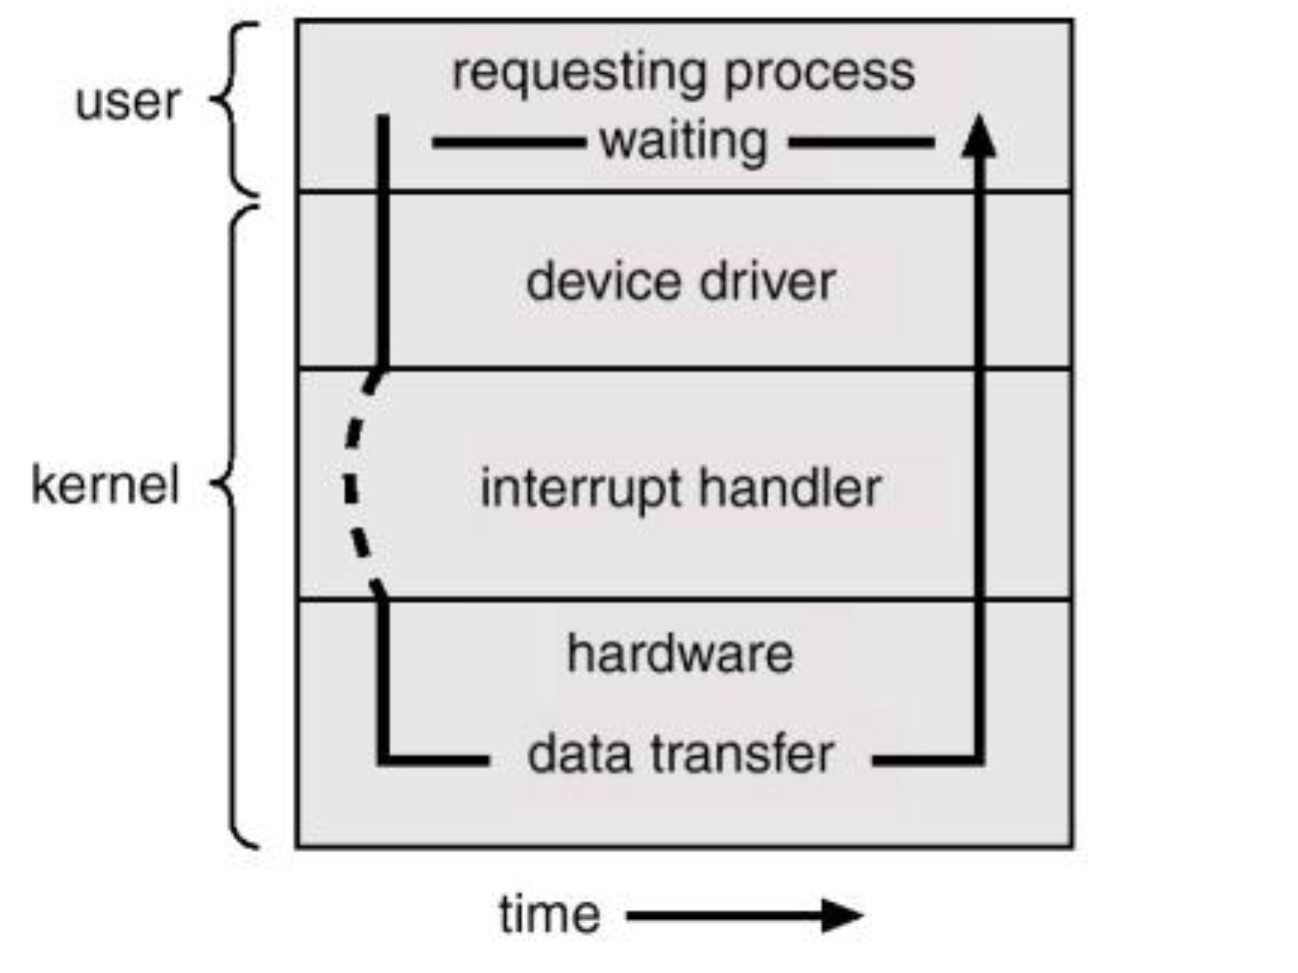
\includegraphics[width=0.8\linewidth]{assets/interrupt-sync.jpeg}
        \caption{Interrupt Sincrono}
    \end{minipage}
    \hspace{0.01\textwidth}
    \begin{minipage}{0.4\textwidth}
        \centering
        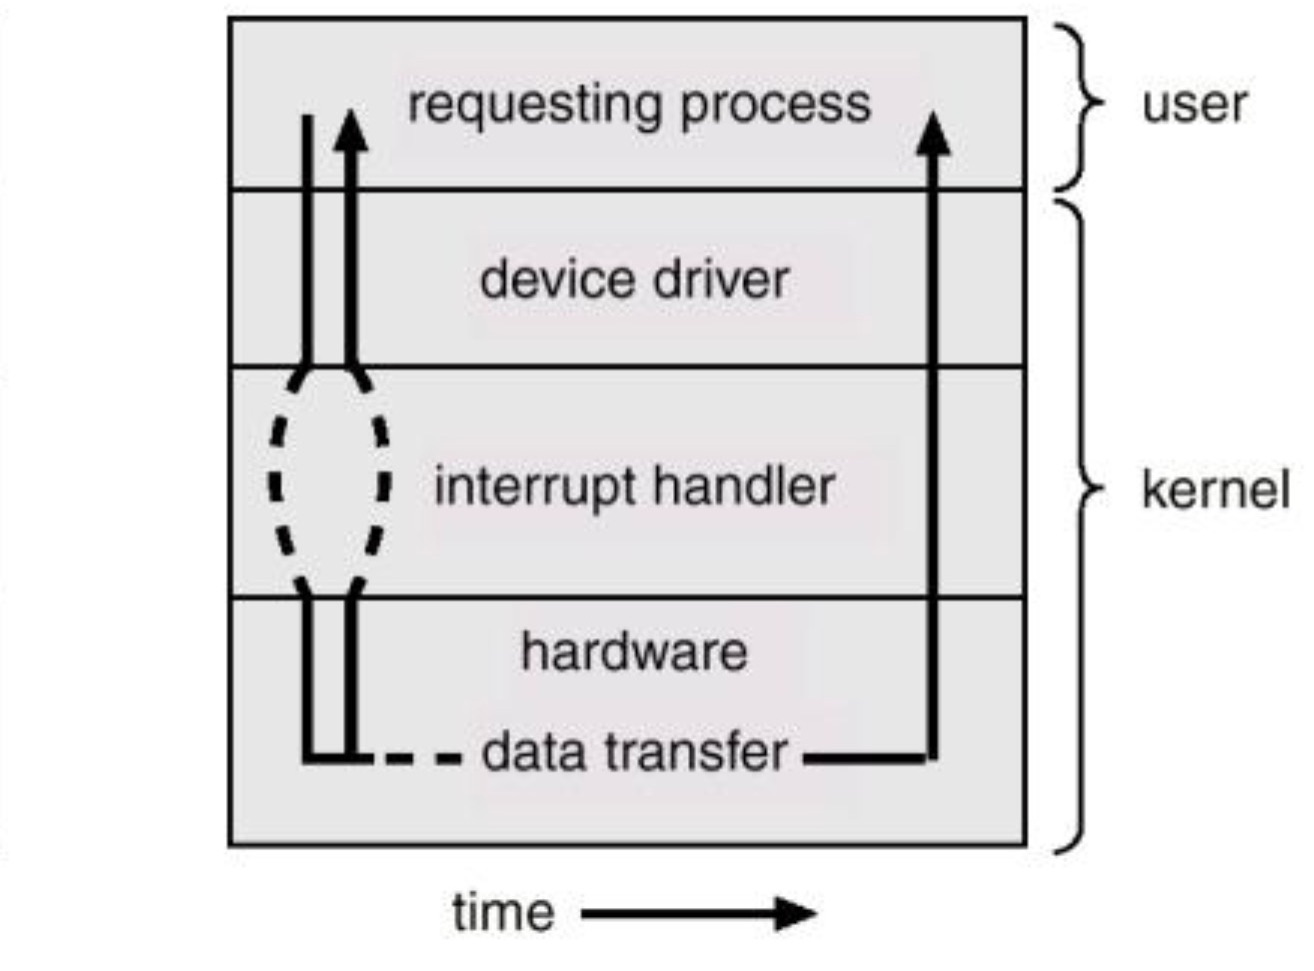
\includegraphics[width=0.8\linewidth]{assets/interrupt-async.jpeg}
        \caption{Interrupt Asincrono}
    \end{minipage}
\end{figure}

\subsubsection{Trap}
Una trap (o eccezione) è un interrupt generato via software, causato da un errore o da una richieste utente (\textit{System Call}).

Le \textit{system call} sono dei meccanismi che possono essere usati da un processo a livello utente o livello applicativo, per richiedere un servizio a livello kernel.


\subsection{DMA}
Il DMA (\textit{Direct Memory Access}) è una strategia che permette di \textbf{trasferire rapidamente grandi quantità di dati}.

\spacer
Dopo che il controller si accorda col il sistema rispetto a dove devono essere scritti i dati in memoria principale, il controller può trasferire interi blocchi di dati senza alcun intervento da parte della CPU.

Viene solo generato un interrupt per ogni blocco trasferito per comunicare che l'operazione è avvenuta con successo.

Utilizzando questa strateglia la CPU è libera di svolgere altre operazioni mentre il controller trasferisce i dati.

\begin{figure}[H]
    \centering
    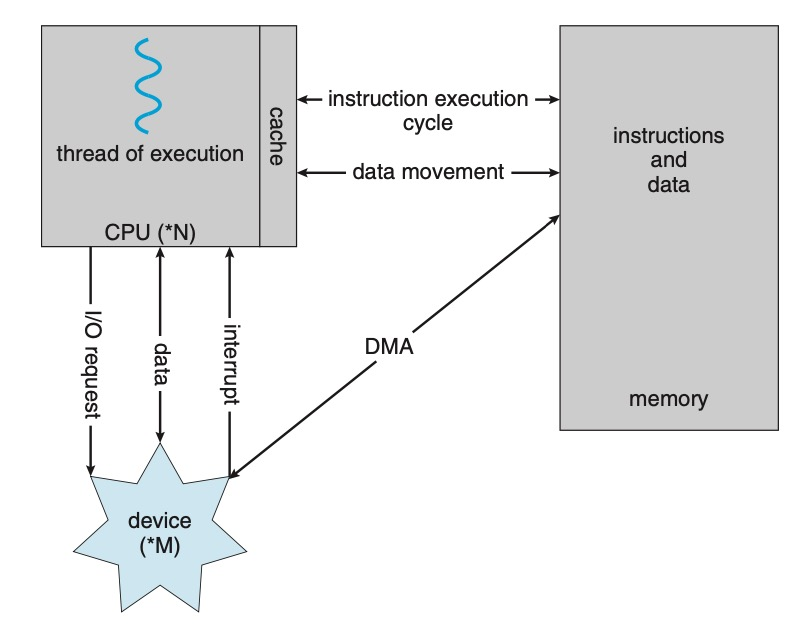
\includegraphics[width=0.45\linewidth]{assets/DMA.jpg}
\end{figure}

\begin{note}
    Esiste anche Remote Direct Memory Access che consente di trasferire dati tra la memoria di due computer, senza sovraccaricare il sistema ricevente.

    Il RDMA è particolarmente utile, se non indispensabile, per processi eseguiti in parallelo tra computer ad alte prestazioni.
\end{note}

\subsection{Operazioni Multimodali}
Proprio come l'hardware anche l'esecuzione del sistema operativo è scandita dagli interrupt. Nel sistema operativo gli interrupt cambiano la modalità di esecuzione dell'hardware.

Tutti i sistemi operativi utilizzano almeno 2 modalità di operazione:
\spacer
\begin{sitemize}
    \item \textbf{User mode:} Modalità dove vengono eseguiti i processi dell'utente, questi processi non hanno completa libertà sul sistema, alcune operazioni sono illegali a questo livello. Se vengono eseguite l'hardware ritorna il controllo al sistema operativo.

    Inoltre anche l'accesso alla memoria ed a altre risorse viene limitato in questa modalità.

    \item \textbf{Kernel mode:} Modalità privilegiata che permette l'accesso completo all'hardware e che viene utilizzata solo dal sistema operativo
\end{sitemize}

\begin{figure}[H]
    \centering
    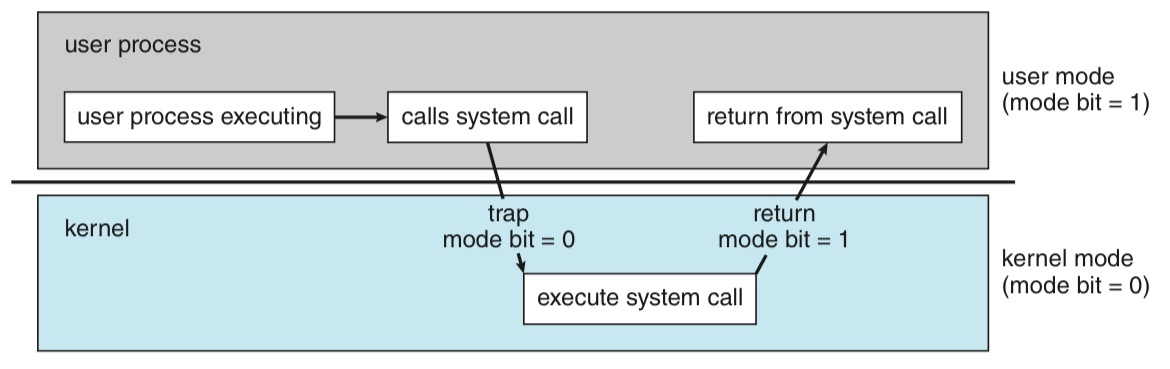
\includegraphics[width=0.65\linewidth]{assets/multimode.jpeg}
\end{figure}

Nelle implementazioni reali vengono utilizzare molte più di 2 modalità, uno tra questi è spesso per le macchine virtuali, mentre altri vengono utilizzati per implementare i livelli di privilegio.

\subsubsection{Timer}
Per prevenire che alcuni processi eseguano cicli infiniti o che semplicemente non restituiscano il controllo al Sistema Operativo gli si fornisce un limite di tempo sull'esecuzione.

Alla creazione di un processo utente si crea anche un timer che se arriva a zero genera un interrupt che ritorna automaticamente il controllo al sistema.
